\documentclass[a4paper, 12pt]{book}
% preamble.tex

\usepackage[utf8]{inputenc}
\usepackage[T1]{fontenc}
\usepackage[english]{babel} % Ho cambiato in italian, supponendo che la maggior parte del testo sia in italiano
\usepackage{amsmath}
\usepackage{amssymb}
\usepackage{graphicx}
\usepackage{hyperref}
\usepackage{geometry}
\usepackage{fontspec} % Utile per Xetex/LuaLaTeX ma mantenuto
\usepackage{booktabs}
\usepackage{amsthm}
\usepackage{enumitem}
\usepackage{caption}
\usepackage{thmtools}
\usepackage{standalone} % Già presente nel tuo elenco
\usepackage{tkz-euclide}
\usepackage{graphicx}
\usepackage[T1]{fontenc}
\usepackage{wesa}

% --- PACCHETTI AGGIUNTI PER LA FORMATTAZIONE ---
\usepackage{parskip}  % Aggiunge spazio tra i paragrafi (stile "blocco")
\usepackage{fancyhdr} % Per intestazioni e piè di pagina personalizzati

% --- IMPOSTAZIONI GEOMETRIA E FONT ---
\geometry{a4paper, margin=1in}

% Configura lo stile 'plain' (usato da \maketitle e \tableofcontents)
% per essere coerente con il piè di pagina
\fancypagestyle{plain}{
    \fancyhf{} % Pulisce
    \cfoot{\thepage} % Mette solo il numero di pagina
    \renewcommand{\headrulewidth}{0pt} % Niente linea su queste pagine
}

% Configurazione Header/Footer per le altre pagine
\pagestyle{fancy}
\fancyhead{} % Pulisce l'intestazione
\fancyfoot{} % Pulisce il piè di pagina
\fancyhead[L]{\nouppercase{\rightmark}} % Nome Sezione a sinistra (o Chapter)
\fancyhead[R]{\nouppercase{\leftmark}}  % Nome Capitolo a destra (o Sezione)
\fancyfoot[C]{\thepage} % Numero di pagina al centro
\renewcommand{\headrulewidth}{0.4pt}
\renewcommand{\footrulewidth}{0pt}


% --- DEFINIZIONI TEOREMI ---
% (Questa parte è cruciale per la tua struttura)
\newtheoremstyle{mythmstyle}%
    {}%
    {}%
    {\itshape}%
    {}%
    {\bfseries}%
    {}%
    { }%
    {\thmname{#1}\thmnumber{ #2}%
    \thmnote{: #3\addcontentsline{toc}{subsubsection}{{\itshape#1}: #3}}. }

% 2. Imposta questo stile come quello ATTUALE
\theoremstyle{mythmstyle}

\newtheorem{theorem}{Th}[section]
\newtheorem{definition}{Def}[section]
\newtheorem{proposition}{Prop}[section]
\newtheorem{corollary}{Cor}[section]
\newtheorem{algorithm}{Alg}[section]
\newtheorem{lemma}{Lemma}[section]
\newtheorem*{remark}{Rem}

% Definizioni utili per il Main file
\newcommand{\inputlesson}[1]{\clearpage\input{#1}\clearpage} % Comando per input lezione

\usepackage{tikz}
\usetikzlibrary{shapes,fit}
\usepackage{amsmath} % Required for align environment
\usepackage{caption} % Required for \captionof outside float environments



\begin{document}
\setcounter{chapter}{10}
\chapter{Lesson 9-12-2025}
\section{Picocell and indoor models}

Generally we have a path loss like (3.8), with $\eta=3.5$.
The shadow fading is usually ranging between 3 and 6dB.

\section{Small-scale fading}

\subsection{Multipath propagation (+Rayleigh and Rice fading)}

\begin{center}
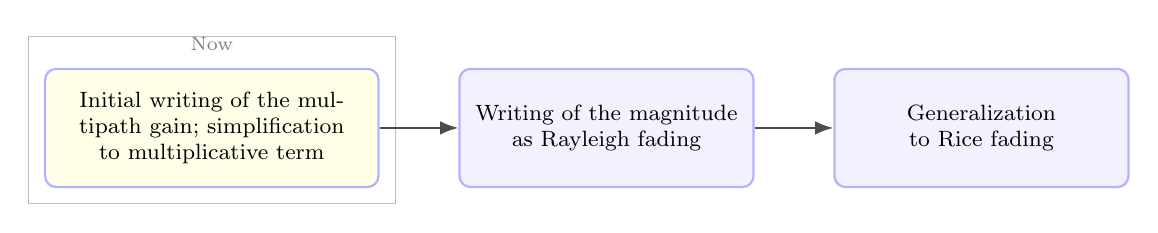
\begin{tikzpicture}[
    node distance=1cm and 1cm,
    box/.style={rectangle, draw=blue!30, rounded corners, align=center, minimum height=1.5cm, font=\footnotesize, thick},
    yellowbox/.style={box, fill=yellow!10},
    purplebox/.style={box, fill=blue!5},
    arrow/.style={-Latex, thick, color=black!70}
]

    % Nodes
    \node[yellowbox, text width=4cm] (start) {Initial writing of the multipath gain; simplification to multiplicative term};
    \node[purplebox, right=of start, text width=3.5cm] (middle) {Writing of the magnitude as Rayleigh fading};
    \node[purplebox, right=of middle, text width=3.5cm] (end) {Generalization to Rice fading};
    
    % Label "Now"
    \node[above=0.1cm of start, font=\scriptsize, color=gray] {Now};
    \draw[gray!50, thin] ($(start.north west)+(-0.2,0.4)$) rectangle ($(start.south east)+(0.2,-0.2)$);

    % Arrows
    \draw[arrow] (start) -- (middle);
    \draw[arrow] (middle) -- (end);

\end{tikzpicture}
\end{center}

\begin{yellowbox}
\faBook\ \textit{Channel modeling (pp. 131-208), page 13}

Let us now zoom in and enter the small-scale realm. When dealing with continuous-time representations, we use the complex \textcolor{green!60!black}{pseudo-baseband channel response}. We also recall from Section 2.2.3 that, \textcolor{green!60!black}{to discretize this representation}, lowpass filtering is in general required before sampling, although in those cases when the discretization returns a singletap response and the effect is only multiplicative, the complex gain of the pseudo-baseband channel can be borrowed directly.
\end{yellowbox}

Due to the various NLOS effects, what the receiver observes is a superposition of a number of replicas of the transmitted signal; the overall channel response is a sum of all these various contributions.

Each path can be described using the attenuation $A_q$ and the delay $\tau_q$, under the form
\begin{align*}
A_q \delta(\tau - \tau_q) e^{-j 2\pi f_c \tau_q} \,.
\end{align*}

\begin{yellowbox}
\faBook\ \textit{Channel modeling (pp. 131-208), page 13}

Since they stem from objects within the local neighborhoods, all the relevant paths can be assumed to be subject to similar pathloss and shadow fading, suitably modified by the local reflection/diffraction/scattering, and thus \textbf{the complex gains $\{A_q\}$ may not exhibit major differences}. However, because at carrier frequencies of
\end{yellowbox}

interest the phase $2\pi f_c \tau_q$ shifts radically with the slightest variation in $\tau_q$, the differences in path delays are always sufficient to regard the path phases as independent random variables.

\begin{yellowbox}
\faBook\ \textit{Channel modeling (pp. 131-208), page 13}

Suppose for now that the transmit signal $x(t)$ corresponds to a passband sinusoid at frequency $f_c$. \textbf{Since the effect of a delay on such a signal is merely a phase shift, we can absorb each delay $\tau_q$ as a shift} $2\pi f_c \tau_q$ in the phase of $A_q$. Then, the overall channel impulse response can be written as

\begin{align}
\underbrace{\left( \sum_q A_q e^{-j 2\pi f_c \tau_q} \right)}_{\text{Gain} = \sqrt{G} \cdot h} \delta(\tau) \,, \tag{3.21}
\end{align}

which is only possible if we eliminate the delay by transforming
\[
\delta(\tau - \tau_q) \to \delta(\tau) \,,
\]
while actually considering only the phase shift caused by the complex exponential.
\end{yellowbox}

\begin{bluebox}[\faPen\ In class]
If we're in the narrowband case (we have a narrow band signal), this means that the symbol duration is much larger than the inverse of the bandwidth.
This means that we have a large symbol, then a delay, the symbols are more or less aligned:

\begin{center}
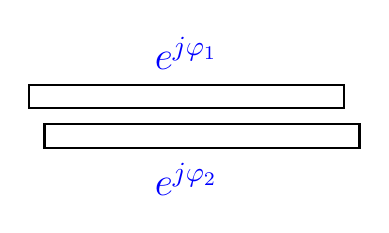
\begin{tikzpicture}
    % Stacked rectangles
    \draw[thick] (0, 0.5) rectangle (4, 0.8);
    \draw[thick] (0.2, 0) rectangle (4.2, 0.3);
    
    % Labels
    \node[text=blue, font=\Large] at (2, 1.2) {$e^{j\varphi_1}$};
    \node[text=blue, font=\Large] at (2, -0.4) {$e^{j\varphi_2}$};
\end{tikzpicture}
\end{center}

We can use the same coefficient but they might have a different phase (blue).
We thus assume we have just one delta and that's where the second summation (the one on the right) comes from.
In this case we have a one tap channel with a gain of $\sqrt{G} \cdot h$. We know $h$ is random but must be either modulus one or variance 1.
This is modeled due to the Central Limit Theorem like a complex Gaussian with $\sigma^2 = 1$. We have that such a random variable is irrotational. The phase varies randomly between 0 and $2\pi$.
\end{bluebox}

% --- FINE PAGINA 15 / INIZIO PAGINA 16 ---
\newpage

The signal reaching the receiver will thus be
\[
y(t) = \sqrt{G} h \cdot x(t) \,.
\]

\begin{yellowbox}
\faBook\ \textit{Channel modeling (pp. 131-208), page 14}

Thus, upon a sinusoid the channel does have \textbf{only a multiplicative effect}, i.e., a complex gain. Furthermore, the preceding consideration on the path phases suggests modeling this gain as a sum of IID random variables; if the number of paths is large enough and some mild conditions are satisfied [221], application of the central limit theorem leads to a complex Gaussian distribution. The result of the sum in (3.21) changes rapidly with the position of both transmitter and receiver: a mere displacement on the order of a wavelength alters the path lengths, and thus the delays thereon, by an amount that shifts the path phases drastically, causing major swings in the sum. Put differently, the paths can add constructively or destructively depending on their relative phases, which are completely modified by small changes in position. The same effect transpires if, instead of a change in position, there is a change in frequency that shifts the phases substantially.
\end{yellowbox}

\begin{yellowbox}
\faBook\ \textit{Channel modeling (pp. 131-208), page 14}

The picture that emerges is thus as follows: the large-scale channel features (pathloss and shadow fading) determine the average channel conditions within the local neighborhood while the small-scale fading determines, subject to that local-average, the instantaneous channel conditions at each position and frequency. This invites decoupling the complex gain in (3.21), namely $\sqrt{G} \cdot h$ where $\sqrt{G}$ determines the local-average received power, $P_r$, as per (3.5), whereas the small-scale fading $h$ is normalized to have unit power. This largely achieves the desired separation between large-scale and small-scale features, yet a mild coupling remains in that certain other parameters of the local small-scale fading, e.g., the Rice factor, may depend on (or be correlated with) the large-scale gain. Ideally, the value of the large-scale features should be taken into account when setting those smallscale parameters, or else there is a danger that the hugely convenient decoupling between large- and small-scale gains entails a loss of relevant information.
\end{yellowbox}

\begin{center}
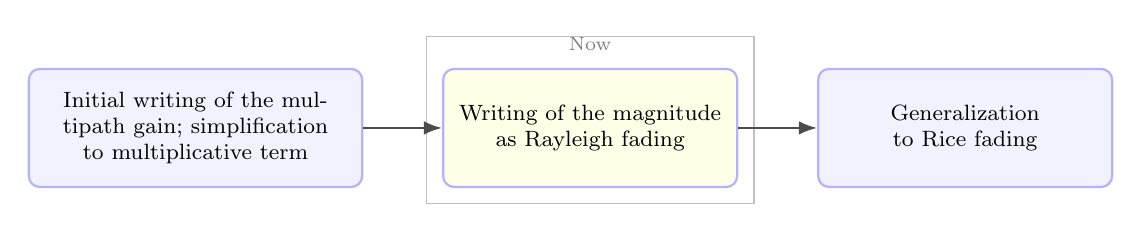
\begin{tikzpicture}[
    node distance=1cm and 1cm,
    box/.style={rectangle, draw=blue!30, rounded corners, align=center, minimum height=1.5cm, font=\footnotesize, thick},
    yellowbox/.style={box, fill=yellow!10},
    purplebox/.style={box, fill=blue!5},
    arrow/.style={-Latex, thick, color=black!70}
]

    % Nodes
    \node[purplebox, text width=4cm] (start) {Initial writing of the multipath gain; simplification to multiplicative term};
    \node[yellowbox, right=of start, text width=3.5cm] (middle) {Writing of the magnitude as Rayleigh fading};
    \node[purplebox, right=of middle, text width=3.5cm] (end) {Generalization to Rice fading};
    
    % Label "Now" moved to the second box
    \node[above=0.1cm of middle, font=\scriptsize, color=gray] {Now};
    \draw[gray!50, thin] ($(middle.north west)+(-0.2,0.4)$) rectangle ($(middle.south east)+(0.2,-0.2)$);

    % Arrows
    \draw[arrow] (start) -- (middle);
    \draw[arrow] (middle) -- (end);

\end{tikzpicture}
\end{center}

The \textbf{small-scale fading is locally modeled as a stationary random process}, in principle zero-mean and complex Gaussian, normalized to have unit variance. At a given position and frequency, then, it is $h \sim \mathcal{N}_{\mathbb{C}}(0,1)$ with \textbf{uniformly distributed phase and with a magnitude that abides by the Rayleigh distribution} (see Appendix C.1.9), hence the popular designation of small-scale fading as simply \textit{Rayleigh fading}. Precisely,

\begin{align}
f_{|h|}(\xi) = \xi e^{-\frac{1}{2}\xi^2} \,, \tag{3.22}
\end{align}

while the power $|h|^2$ follows the exponential distribution

\begin{align}
f_{|h|^2}(\xi) = e^{-\xi} \,, \tag{3.23}
\end{align}

which of course is only defined for $\xi \ge 0$.

\vspace{1em}

\begin{center}
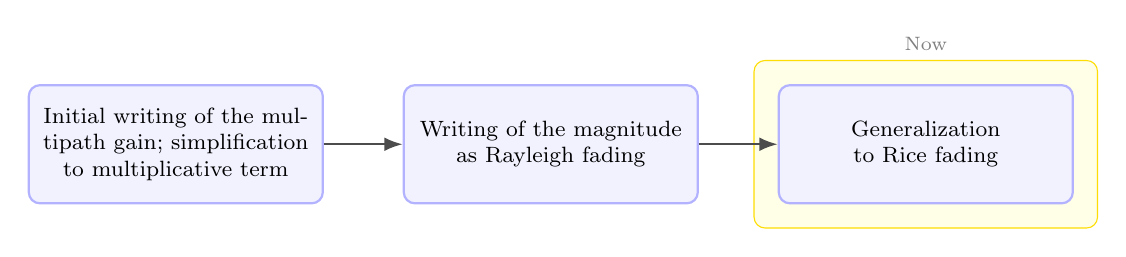
\begin{tikzpicture}[
    node distance=1cm and 1cm,
    box/.style={rectangle, draw=blue!30, rounded corners, align=center, minimum height=1.5cm, font=\footnotesize, thick, fill=blue!5},
    highlight/.style={rectangle, draw=yellow!80!orange, fill=yellow!10, inner sep=0.3cm, rounded corners},
    arrow/.style={-Latex, thick, color=black!70}
]

    % Nodes
    \node[box, text width=3.5cm] (step1) {Initial writing of the multipath gain; simplification to multiplicative term};
    \node[box, right=of step1, text width=3.5cm] (step2) {Writing of the magnitude as Rayleigh fading};
    \node[box, right=of step2, text width=3.5cm] (step3) {Generalization to Rice fading};
    
    % Yellow highlight box for the "Now" step (Step 3)
    \node[highlight, fit=(step3)] (hl) {};
    \node[above=0.0cm of hl, font=\scriptsize, color=gray] {Now};

    % Redraw step3 on top to ensure text is visible
    \node[box, text width=3.5cm] at (step3) {Generalization to Rice fading};

    % Arrows
    \draw[arrow] (step1) -- (step2);
    \draw[arrow] (step2) -- (step3);

\end{tikzpicture}
\end{center}

If a multipath term dominates over the rest, e.g., because it propagates through LOS and it is subject to a distinct pathloss, then the receiver can lock onto that signal component and render it \textbf{unfaded}. It follows that $h \sim \mathcal{N}_{\mathbb{C}}(\mu_h, \sigma_h^2)$ with mean $\mu_h \neq 0$ and with variance $\sigma_h^2 = 1 - |\mu_h|^2$. For this \textbf{so-called Rice fading}, we have

\begin{align}
f_{|h|}(\xi) = 2(K+1)\xi e^{-(K+1)\xi^2 - K} I_0 \left( 2\sqrt{K(K+1)}\xi \right) \,, \tag{3.24}
\end{align}

where $K = |\mu_h|^2 / \sigma_h^2$ is the \textbf{Rice factor} while $I_0(\cdot)$ is the zero-order modified Bessel function of the first kind.

\begin{bluebox}[\faPen\ In class]
The K factor is the ratio between the mean signal strength and the variance of a random component.
\end{bluebox}

\textbf{For $K=0$, Rice fading reverts to Rayleigh fading}; for $K \to \infty$, the \textbf{fading vanishes as the value of $h$ becomes deterministic}. Thus, the Rice distribution bridges these extremes and allows, through K, to regulate the severity of the fading. Analytically speaking, however, the PDF in (3.24) is not particularly friendly because of the presence of $I_0(\cdot)$.

\begin{greenbar}
We can't calculate the Bessel functions!
\end{greenbar}

\begin{purplebox}[\faStickyNote\ Mynote]
As it is clear, the distribution of the modulus of the channel $|h|$ is described by (3.24).
\end{purplebox}

A more tractable distribution is the Nakagami-m distribution, see \textcolor{green!60!black}{08.3\_pp\_131\_208\_Channel\_modeling, page 15}.

There are other magnitude distribution; generally Ricean is used when we don't have a direct line of sight.

% --- FINE PAGINA FADING / INIZIO PAGINA DIGRESSIONE ---
\newpage

\section[Importance of channel modeling]{Digression on the importance of channel modeling, standardization institutions}

\begin{greenbar}
We were talking about the channel models; a few words before the actual lecture: tomorrow we'll have a regular lecture.
\end{greenbar}

\textbf{About this chapter}: in general there's not a well-shaped channel modeling theory; if we feel we're confused, it's normal at the first approach. At the beginning we said we're trying to make a mathematical model for a really complicated environment: to make a deterministic model for such a situation would be too difficult by far.
We resorted to models which should mimic reality. Unfortunately, we don't have an agreed model; for the noise, we know that we have WGN. Here we have a confusing situation: what we want to design depends on our purpose; we have models which are useful in certain situations, other models which are useful in certain others.
Specifically, we're looking for the limits of our systems; when we know what the ultimate limit is, we know how far we are from that ultimate limit.
If we are at 3dB from the ultimate performance, there's room for improvement: our effort can pay off. If we're 0.01dB from the limit, our work is done from an engineering perspective; even if we improve, we're really close to the theoretical limit.

When we approach this chapter, we know we have many different models; some are useful (e.g.: a model has gaussian variables as an input of the system). In specific cases we don't have gaussian values, though.

\noindent\rule{\textwidth}{0.4pt}

Important point is that we have very different models depending on what we're doing.
In this chapter we also find practical stuff btw. When we talk about LTE and 5G, who defines what those are?
\textbf{Standardization} is really complicated; internet standards is handled by the IETF (Internet Engineering Task Force): it establishes protocols. Other things standardized are how the wireless network is done and how different networks can communicate; what most interests us is the communication interface: there must be a precise standard to allow communication between different towers etc etc; this is called \textit{radio interface}.
There must be a document saying how we transmit every single bit; we want to have a competitive market, in which multiple brands can improve on the communication.

\begin{greenbar}
In the past, mobile phones were chosen depending on reception capabilities; now we have a field so high that it's very easy to receive signal.
\end{greenbar}

We need to have specifications about sending bits from the central tower to a mobile device and vice versa.
There is not a specification on how the mobile phone should be made, but rather only on how the phone should communicate.

If we know how bits are sent downlink, we might think to use ZF or even better, LMMSE; it must be specified how bits are sending data to the base stations.
We can make base stations however we want: we're the ones deciding the compromise between cost and performance.

% --- FINE PAGINA DIGRESSIONE / INIZIO CONTINUAZIONE DIGRESSIONE E SPACE SELECTIVITY ---
\newpage

For cellular standards we have 3GPP, which is third generation \colorbox{yellow!40}{??} program. How can we participate in specification of 3GPP? We can't do that easily: it's made by several regional standard organizations; here in Europe we have ETSI (European Telecommunications Standard Institute). In Japan we have ARIB, \dots
Who is member of those partners can send standards to 3GPP; we can be members if we pay a fee, which depends on turnover of company, \dots; in the 3GPP is dealing with radio access networks. How do they decide if we use OFDM or whatever?

\begin{greenbar}
3: why? 1: analog, 2: GSM, 3: after GSM, 4: LTE, 5G, 6G, \dots
\end{greenbar}

2G was specified by ETSI and adopted by other countries. For 3G they wanted to have global roaming; that's how 3GPP was formed.
It was decided that 3G would use WCDMA (Wideband CDMA). Let's suppose we have different technologies.
Today we have OTFS, which is a way to transmit bits; how do we decide in a group which of the various options we have is better? What happens is that we do theoretical simulations; in all of this exercise there is a critical point: which channel model do we use? Depending on the model, it might happen that a technology is better than another; an initial debate was in fact on which channel model should have been used. The first thing we need to do when developing standards is agreeing on the channel model.

\begin{greenbar}
In section 3.8 we'll find MIMO in standards.
\end{greenbar}

Different groups adapt different models; there are researches being made on identifying good and representative channel models.

Professor advises us to go through the chapter and then go back and redo it, since the picture will be much clearer. We cannot forget reality; at the same time, we're doing something inspired by reality.

\section{Space selectivity}

\begin{bluebox}[\faPen\ In class]
We have a factor modulating the straight path and the other paths; the average of the sum is given by the straight, while the average of the power is given by considering all.

\begin{center}
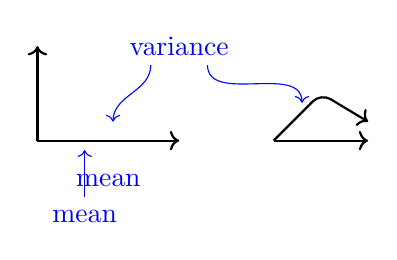
\begin{tikzpicture}[scale=1.2]
    % Vectors
    \draw[thick, ->] (0,0) -- (1.5,0) node[midway, below=0.3cm, text=blue] {mean};
    \draw[thick, ->] (0,0) -- (0,1);
    
    % Wiggly line for variance
    \draw[thick, ->, rounded corners] (2.5,0) -- (3.5,0);
    \draw[thick, ->, rounded corners] (2.5,0) -- (3,0.5) -- (3.5,0.2);
    
    % Labels (Blue handwriting style)
    \node[text=blue] at (1.5, 1) {variance};
    \draw[blue, ->] (1.2, 0.8) to[out=270, in=90] (0.8, 0.2); % Arrow pointing to vertical component
    \draw[blue, ->] (1.8, 0.8) to[out=270, in=90] (2.8, 0.4); % Arrow pointing to random component
    
    \node[text=blue] at (0.5, -0.8) {mean};
    \draw[blue, ->] (0.5, -0.6) -- (0.5, -0.1);
\end{tikzpicture}
\end{center}

Space selectivity; we need somehow to have this. the two locations could be the
\end{bluebox}
% --- INIZIO PAGINA NOTE MANOSCRITTE (Space Selectivity) ---
\newpage

locations of the two antennas; let's say we have a wave which is hitting the two antennas:

\begin{figure}[h]
    \centering
    % [IMAGE PLACEHOLDER: Diagram of Transmitter, Scatterer, Diffraction, Reflection, Receiver 0/1]
    
\includegraphics[width=0.8\textwidth]{Pictures/image copy 2.png}
\end{figure}

We know that if we go far the curvature is almost null.

\begin{center}
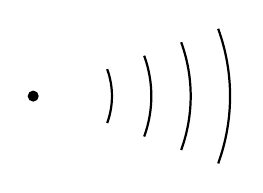
\begin{tikzpicture}
    % Source point
    \fill (0,0) circle (2pt);
    
    % Expanding waves
    \foreach \r in {1, 1.5, 2, 2.5} {
        \draw[thick] (20:\r) arc (20:-20:\r);
    }
    
\end{tikzpicture}
\end{center}

There is a difference of length at various points: this will also mean we have a difference in phase.
This difference matters a lot; this means that \textbf{selectivity stays not in frequency, but in space}.
In the previous drawing we might have a phase perfect and a non-in-phase signal: we can't just sum them, otherwise we'd have a problem.
We might have scattering clusters, if we don't do anything.
There are many resons to have space selectivity. We also have a PAS, but we'll see it next week.
We know the spectrum of the signal tells us how the power is distributed on the various frequencies.
If we talk about Power Angle, we talk about distribution depending on the angulation of transmission. This is what PAS means.

In the previous drawing we were in a 2-d setting; we live in a 3-d setting; we should consider not only the azimuth but also the elevation.
Generally we don't have influence in the elevation, while we have a lot of influence if we change the azimuth.

% --- FINE NOTE MANOSCRITTE / INIZIO PAGINA 08 ---
\newpage

\section{PAS $\to$ Power Angle Spectrum}

\textbf{What's the PAS?}
\begin{align*}
\text{PAS}(\theta) &\to \text{function} \\
\text{TX func} &\to \text{RX func} \\
\text{RX power} &= \text{PAS}(\theta) \times \text{Tx power}
\end{align*}

\begin{greenbar}
\textbf{From the book:}
The \textbf{phase shifts} between different locations we referred to in equations such as (3.21), are governed, at least \textbf{in the local neighborhood}, by the angle between the propagation paths and the segment connecting those locations, as can be seen in the figure (which shows the segment connecting two locations with a propagation path at an angle $\theta$):
\end{greenbar}

\begin{figure}[h]
    \centering
    % [IMAGE PLACEHOLDER: Diagram of Transmitter, Scatterer, Diffraction, Reflection, Receiver 0/1]
    
\includegraphics[width=0.9\textwidth]{Pictures/image.png}
\end{figure}

The change of path length between the two is simple given by $\Delta_D \cos(\theta)$, aka by projecting the segment on the path direction.

\begin{bluebox}[\faPen\ Power Angle Spectrum (PAS)]
Since \textbf{the projection depends on $\theta$}, it is \colorbox{yellow!30}{crucial to have a function which establishes} the \textbf{angular distribution of paths}; this function is the PAS (Power Angle Spectrum), which \colorbox{yellow!30}{expresses the received signal power as a function of angle when acting as a} \colorbox{yellow!30}{receiver}; instead, when we're acting as a transmitter, instead, the PA expresses the transmitted signal power that reaches the receiver at the other end of the link as a function of the angle of departure.
\end{bluebox}

\begin{yellowbox}
\faBook\ \textit{Channel modeling (pp. 131-208), page 16}

The PAS is a continuous function of angle, \textbf{normalized so it can be interpreted as a PDF}, which is a definition consistent with the unit-power normalization of the small-scale fading.
\end{yellowbox}

The standard deviation of the PAS, viewed as a distribution, gives the root-mean-square (RMS) \textbf{angle spread}.

\begin{yellowbox}
\faBook\ \textit{Channel modeling (pp. 131-208), page 16}

Although, in principle, the definition of the PAS as a continuous function of angle models a diffuse propagation scenario, it does not preclude modeling \textbf{situations where}

\textbf{power is received only from a finite number of discrete angles}; these situations can be accommodated by constructing the PAS on the basis of discrete delta functions. Formally, the PAS is a function of both azimuth and elevation. However, empirical measurements have indicated that in most outdoor wireless systems the dependence on elevation plays only a secondary role [224]. Historically then, the focus has been on characterizing the marginal PAS on the azimuth plane—in fact, PAS can also be taken to stand for power azimuth spectrum—yet the elevation dimension should not be carelessly dismissed in other types of deployment, e.g., indoors or in vertical urban picocells. We return to this aspect at the end of the chapter. Several functions have been proposed and applied to model the marginal PAS in azimuth, which in this text is denoted by $\mathcal{P}(\cdot)$.
\end{yellowbox}

\begin{greenbar}
\textbf{In class:} \\
Last lesson, we were talking about space selectivity. We talk about it because we may have 2 (or more) antennas: a part of the signal might be traveling a larger distance; in our case, it is $\Delta_D \cos(\theta)$.

\begin{center}
    % [IMAGE PLACEHOLDER: Diagram of Transmitter, Scatterer, Diffraction, Reflection, Receiver 0/1]
    
\includegraphics[width=0.5\textwidth]{Pictures/image copy.png}
\end{center}

Normally, this is not so big that the strength of signal goes down, but the phase may change. If we apply a phase shift on location 1, it's like as if we made the signal \textit{start late}. We can steer the wave with different angles by changing the phase of a certain amount. This is the intuition behind what happens when a certain wave is hitting the two antennas. If we have multiple antennas, we just apply the same principle.
We can thus make the antenna sensitive to a certain direction: even if we have an omnidirectional antenna, the Power Angle Spectrum is modeling the fact that if we have an antenna, we might have waves coming from multiple directions
\end{greenbar}

% --- INIZIO PAGINA 10 (HANDWRITTEN NOTES) ---
\newpage

\begin{center}
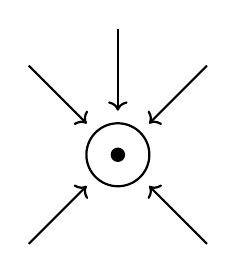
\begin{tikzpicture}[scale=0.8]
    % Central dot
    \filldraw (0,0) circle (3pt);
    \draw[thick] (0,0) circle (0.5cm);
    
    % Arrows pointing inwards
    \foreach \angle in {45, 135, 225, 315} {
        \draw[thick, ->] (\angle:2cm) -- (\angle:0.7cm);
    }
    \draw[thick, ->] (90:2cm) -- (90:0.7cm);
\end{tikzpicture}
\end{center}

What do we do in such a situation? The PAS is a probability distribution which tells where it's most likely that the signal is arriving.

\begin{center}
\begin{tikzpicture}[scale=1.0]
    % Axes
    \draw[thick] (0,0) -- (4,0);
    \draw[thick] (0,0) -- (0,1);
    \draw[thick] (4,0) -- (4,1);
    
    % Ticks
    \node[below] at (0,0) {0};
    \node[below] at (2,0) {$\pi$};
    \node[below] at (4,0) {$2\pi$};
    \draw[thick] (2, 0.1) -- (2, -0.1);
    
    % Curve
    \draw[thick] (0, 0.5) to[out=20, in=180] (2, 1.2) to[out=0, in=160] (4, 0.5);
    
    % Hatching
    \fill[pattern=north east lines, pattern color=black] (0,0.5) to[out=20, in=180] (2, 1.2) to[out=0, in=160] (4, 0.5) -- (4,0) -- (0,0) -- cycle;
\end{tikzpicture}
\end{center}

We don't need to confuse the word \textit{spectrum} being used here: we're not talking about frequencies!

\begin{center}
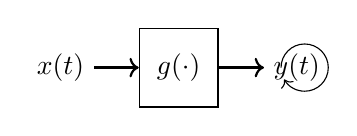
\begin{tikzpicture}[node distance=1.5cm]
    % Block diagram
    \node (input) {$x(t)$};
    \node[draw, minimum width=1cm, minimum height=1cm, right of=input] (sys) {$g(\cdot)$};
    \node[right of=sys] (output) {$y(t)$};
    
    \draw[->, thick] (input) -- (sys);
    \draw[->, thick] (sys) -- (output);
    
    % Circular arrow on output?
    \draw[->] (2.8, 0) arc (180:-150:0.3);
\end{tikzpicture}
\end{center}

\begin{align*}
P_y(f) = |G(f)|^2 P_x(f)
\end{align*}

\begin{center}
\begin{tikzpicture}[scale=0.8]
    % Curve small
    \draw[thick] (0,0) -- (4,0);
    \draw[thick] (0, 0.2) to[out=10, in=180] (2, 0.8) to[out=0, in=170] (4, 0.2);
    \fill[pattern=north east lines] (1,0) -- (1, 0.6) to[out=20, in=160] (3, 0.6) -- (3,0) -- cycle;
\end{tikzpicture}
\end{center}

This allows us to understand where we can capture more energy. The PAS tells where we have more power depending on the angle.

% --- FINE PAGINA 10 / INIZIO PAGINA 11 ---
\begin{figure}[h]
    \centering
    % [IMAGE PLACEHOLDER: Diagram of Transmitter, Scatterer, Diffraction, Reflection, Receiver 0/1]
    
\includegraphics[width=0.5\textwidth]{Pictures/image copy 3.png}
\end{figure}

Antennas are generally 30m high and have a tilting on their top of a few degrees:

\begin{center}
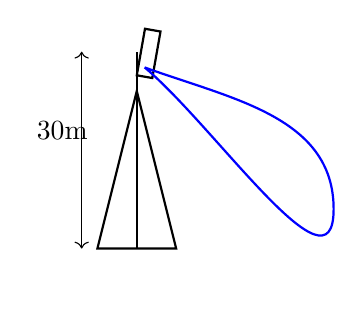
\begin{tikzpicture}
    % Tower
    \draw[thick] (0,0) -- (0.5, 2) -- (1,0) -- cycle;
    \draw[thick] (0.5, 0) -- (0.5, 2.5); % Pole
    
    % Antenna element
    \draw[thick, rotate around={-10:(0.5, 2.2)}] (0.5, 2.2) rectangle (0.7, 2.8);
    
    % Beam lobe
    \draw[blue, thick] (0.6, 2.3) to[out=-20, in=90] (3, 0.5) to[out=-90, in=-40] (0.6, 2.3);
    
    \node[left] at (0, 1.5) {30m};
    \draw[<->] (-0.2, 0) -- (-0.2, 2.5);
\end{tikzpicture}
\end{center}

we need to decide the tilting depending on the application we want to have.

If we have a motor wave we have a central base station and then smaller others. If a network sees we're jumping, it will assign us to an umbrella base station: the probability that the calls drop is lower.

\begin{center}
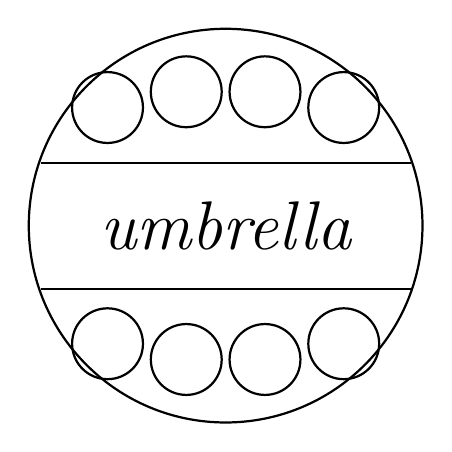
\begin{tikzpicture}[scale=1.0, transform shape]
    % 1. Cerchio esterno (Macrocella)
    \draw[thick] (0,0) circle (2.5cm);

    % 2. Linee divisorie orizzontali (Banda centrale)
    \draw[thick] (-2.35, 0.8) -- (2.35, 0.8);
    \draw[thick] (-2.35, -0.8) -- (2.35, -0.8);

    % 3. Testo "umbrella"
    % Uso il corsivo e una dimensione adeguata
    \node[font=\fontsize{30}{40}\selectfont\itshape] at (0, 0) {umbrella};

    % 4. Cerchi superiori (Microcelle) - INTERNI
    % Ho abbassato la Y e stretto la X per farli stare dentro
    \draw[thick] (-1.5, 1.5) circle (0.45cm);
    \draw[thick] (-0.5, 1.7) circle (0.45cm);
    \draw[thick] (0.5, 1.7) circle (0.45cm);
    \draw[thick] (1.5, 1.5) circle (0.45cm);

    % 5. Cerchi inferiori (Microcelle) - INTERNI
    % Speculari a quelli sopra
    \draw[thick] (-1.5, -1.5) circle (0.45cm);
    \draw[thick] (-0.5, -1.7) circle (0.45cm);
    \draw[thick] (0.5, -1.7) circle (0.45cm);
    \draw[thick] (1.5, -1.5) circle (0.45cm);

\end{tikzpicture}
\end{center}

\textbf{Clarke-Jakes PAS} $\to$ take it as example.

We have various examples of PAS; Clarke-Jakes' is a uniform one:

\textcolor{red}{Possible question: what is a PAS?}

% --- FINE PAGINA 11 / INIZIO PAGINA 12 ---


\begin{center}
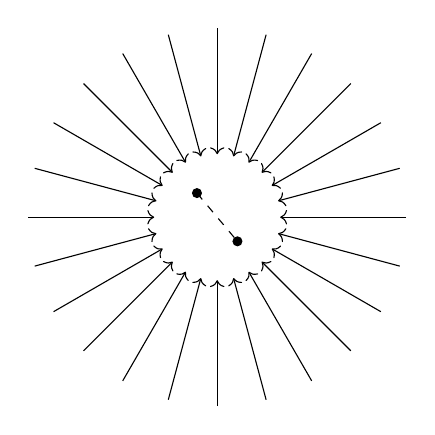
\begin{tikzpicture}[scale=0.8]
    % Clarke-Jakes Starburst
    \foreach \angle in {15, 30, ..., 360} {
        \draw[->] (\angle:3cm) -- (\angle:1cm);
    }
    
    % Two dots
    \filldraw (130:0.5cm) circle (2pt);
    \filldraw (-50:0.5cm) circle (2pt);
    
    % Dashed line
    \draw[dashed] (130:0.5cm) -- (-50:0.5cm);
    
\end{tikzpicture}
\end{center}

With
\begin{align}
\mathcal{P}(\theta) = \frac{1}{2\pi} \quad \theta \in [-\pi, \pi) \tag{3.27}
\end{align}

\begin{yellowbox}
\faBook\ \textit{Channel modeling (pp. 131-208), page 16}

It fits surprisingly well the behavior observed at mobile users, capturing the essence of multipath propagation in a manner that is friendly to analysis. Such friendliness, however, drops markedly as soon as the angular range is reduced below $2\pi$ and more convenient alternatives exist if directional preference (particularly important in transceivers located above the clutter, e.g., elevated base stations) is to be introduced.
\end{yellowbox}

The \colorbox{yellow!30}{Clarke-Jakes PAS is widely used}. There are other spectrums related to this one, but it shall not be confused with stuff about the delay.

\section{Truncated Laplacian}

We may use another $\mathcal{P}(\theta)$, the Truncated Laplacian.

\begin{center}
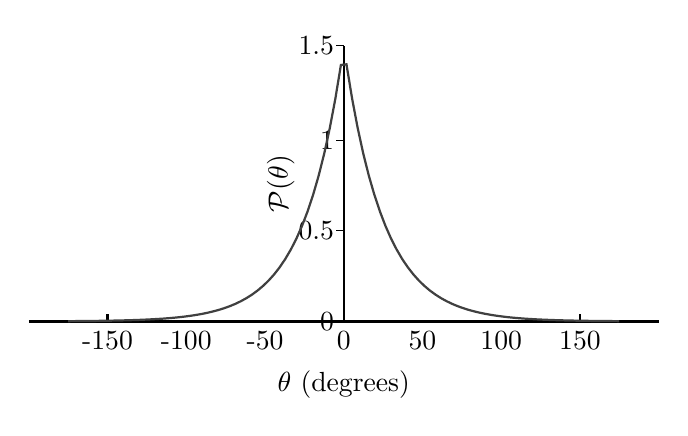
\begin{tikzpicture}[scale=1.0]
    % Axes
    \draw[thick] (-4,0) -- (4,0);
    \draw[thick] (-3,0) -- (-3, 0.1); % tick
    \draw[thick] (3,0) -- (3, 0.1); % tick
    \draw[thick] (0,0) -- (0, 3.5);
    
    % Ticks labels
    \node[below] at (-3,0) {-150};
    \node[below] at (-2,0) {-100};
    \node[below] at (-1,0) {-50};
    \node[below] at (0,0) {0};
    \node[below] at (1,0) {50};
    \node[below] at (2,0) {100};
    \node[below] at (3,0) {150};
    \node[below] at (0,-0.5) {$\theta$ (degrees)};
    
    % Y Axis
    \node[left] at (0, 3.5) {1.5};
    \draw (0, 3.5) -- (-0.1, 3.5);
    \node[left] at (0, 2.3) {1};
    \draw (0, 2.3) -- (-0.1, 2.3);
    \node[left] at (0, 1.15) {0.5};
    \draw (0, 1.15) -- (-0.1, 1.15);
    \node[left] at (0,0) {0};
    
    \node[rotate=90] at (-0.8, 1.75) {$\mathcal{P}(\theta)$};
    
    % Laplacian Curve (Approx)
    \draw[thick, darkgray] plot[domain=-3.5:3.5, samples=100] (\x, {3.5 * exp(-2*abs(\x))});

\end{tikzpicture}
\end{center}

% --- INSERIMENTO FORMULE TRUNCATED LAPLACIAN (da immagine.png) ---

With
\begin{align}
\mathcal{P}(\theta) = \frac{K_L}{\sqrt{2}\sigma_\theta} \exp \left( - \left| \frac{\sqrt{2}(\theta - \mu_\theta)}{\sigma_\theta} \right| \right) \,, \quad \theta \in [\mu_\theta - \pi, \mu_\theta + \pi) \tag{3.32}
\end{align}

where $K_L$ is a factor which makes the integral be 1, thus defined as

\begin{align}
K_L = \frac{1}{1 - \exp(-\sqrt{2}\pi/\sigma_\theta)} \,. \tag{3.33}
\end{align}

\vspace{2em}
\noindent\rule{\textwidth}{1pt}
\vspace{2em}

% --- INSERIMENTO NOTE PAGINA 01 (Small-scale fading notes) ---

\section{Small-scale fading}

\subsection{Multipath propagation (+Rayleigh and Rice fading)}

\begin{center}
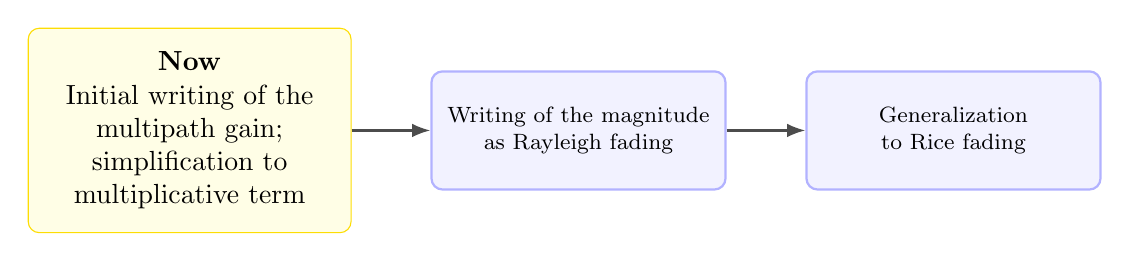
\begin{tikzpicture}[
    node distance=1cm and 1cm,
    box/.style={rectangle, draw=blue!30, rounded corners, align=center, minimum height=1.5cm, font=\footnotesize, thick, fill=blue!5},
    highlight/.style={rectangle, draw=yellow!80!orange, fill=yellow!10, inner sep=0.3cm, rounded corners},
    arrow/.style={-Latex, thick, color=black!70}
]
    % Flowchart reconstruction
    \node[highlight] (step1) {
        \begin{minipage}{3.5cm}
        \centering
        \textbf{Now}\\
        Initial writing of the multipath gain; simplification to multiplicative term
        \end{minipage}
    };
    \node[box, right=of step1, text width=3.5cm] (step2) {Writing of the magnitude as Rayleigh fading};
    \node[box, right=of step2, text width=3.5cm] (step3) {Generalization to Rice fading};
    
    \draw[arrow] (step1) -- (step2);
    \draw[arrow] (step2) -- (step3);
\end{tikzpicture}
\end{center}

\begin{yellowbox}
\faBook\ \textit{Channel modeling (pp. 131-208), page 13}

Let us now zoom in and enter the small-scale realm. When dealing with continuous-time representations, we use the complex \textcolor{green!60!black}{pseudo-baseband channel response}. We also recall from Section 2.2.3 that, \textcolor{green!60!black}{to discretize this representation}, lowpass filtering is in general required before sampling, although in those cases when the discretization returns a singletap response and the effect is only multiplicative, the complex gain of the pseudo-baseband channel can be borrowed directly.
\end{yellowbox}

\begin{purplebox}[\faQuestionCircle\ My questions]
\textbf{Question:} why we like to work in pseudo baseband? \\
\textbf{Refers to:} \textit{pseudo-complex baseband} $\to$ (what is this?)
\end{purplebox}

Due to the various NLOS effects, what the receiver observes is a superposition of a number of replicas of the transmitted signal; the overall channel response is a sum of all these various contributions.

Each path can be described using the attenuation $A_q$ and the delay $\tau_q$, under the form
\begin{align*}
A_q \delta(\tau - \tau_q) e^{-j 2\pi f_c \tau_q} \,.
\end{align*}

\end{document}